% Methodologie/SectionData.tex


\subsection{Données}

\subsubsection{Source des Données}

Les données utilisées dans cette étude proviennent d'un ensemble de critiques sur des produits alimentaires provenant d'Amazon. Ce jeu de données couvre une période de plus de 10 ans, comprenant l'ensemble des ~500,000 critiques jusqu'en octobre 2012. Les critiques incluent des informations sur les produits et les utilisateurs, les évaluations et une critique en texte brut. De plus, il englobe des critiques de toutes les autres catégories d'Amazon.

Le lien vers les données est disponible sur Kaggle :  \url{https://www.kaggle.com/snap/amazon-fine-food-reviews}.

\subsubsection{Les composants d'un avis}
\begin{figure}[h]
    \centering
    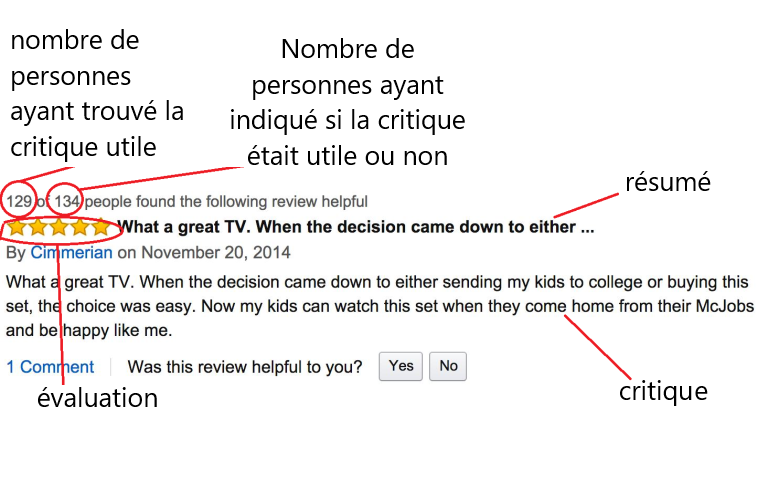
\includegraphics[scale=0.5]{assets/amazonReviewDetails.png}
    \caption{Les elements d'un avis}
    \label{fig:avis}
\end{figure}

Un avis typique de cet ensemble de données comprend plusieurs composants essentiels qui fournissent une perspective détaillée sur l'expérience de l'utilisateur. Voici une énumération des principaux éléments d'un avis dans cet ensemble de données :

1. \textbf{Identifiant Unique ('Id'):} Chaque avis est associé à un identifiant unique, permettant une référence spécifique.

2. \textbf{Code Produit ('ProductId'):} Indique le produit concerné par l'avis, facilitant l'association aux références produits.

3. \textbf{Identifiant de l'Utilisateur ('UserId'):} Identifie de manière unique l'utilisateur ayant publié l'avis.

4. \textbf{Nom du Profil de l'Utilisateur ('ProfileName'):} Le nom du profil associé à l'utilisateur, fournissant un contexte sur l'auteur de l'avis.

5. \textbf{Utilité ('HelpfulnessNumerator' et 'HelpfulnessDenominator'):} Deux valeurs numériques indiquant le nombre d'utilisateurs qui ont trouvé l'avis utile par rapport au nombre total d'évaluations de son utilité.

6. \textbf{Notation ('Score'):} La notation attribuée par l'utilisateur, quantifiant l'appréciation globale du produit.

7. \textbf{Timestamp de l'Avis ('Time'):} La date et l'heure à laquelle l'avis a été publié, offrant une dimension temporelle.

8. \textbf{Résumé ('Summary'):} Un condensé du contenu de l'avis, fournissant une vue d'ensemble rapide.

9. \textbf{Texte Intégral de l'Avis ('Text'):} Le contenu complet de l'avis, offrant des détails contextuels sur l'expérience de l'utilisateur.

Chacun de ces éléments joue un rôle spécifique dans la caractérisation de l'avis, permettant une analyse approfondie des sentiments exprimés dans les avis sur les produits alimentaires de la plateforme Amazon.

\subsubsection{Informations générales sur la dataset}
\begin{figure}[h]
    \centering
    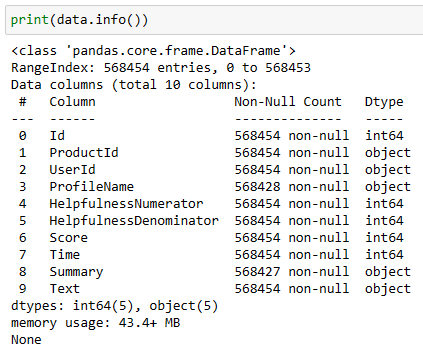
\includegraphics[scale=1]{assets/datainfo.PNG}
    \caption{Les information sur la DataSet}
    \label{fig:dataframeinfo}
\end{figure}
\newpage
La sortie de la fonction \texttt{data.info()} fournit une vue détaillée de la structure de notre ensemble de données. Notre ensemble de données est représenté sous la forme d'un objet de type \texttt{pandas.core.frame.DataFrame}, avec un index de type \texttt{RangeIndex}, allant de 0 à 568453, indiquant ainsi le nombre total d'entrées (lignes) dans la base de données. Il est composé de 10 colonnes au total.

Les attributs et types de données de chaque colonne sont les suivants :
\begin{itemize}
    \item \texttt{'Id'} est de type \texttt{int64} avec 568454 valeurs non nulles.
    \item \texttt{'ProductId'} est de type \texttt{object} (généralement une chaîne de caractères) avec 568454 valeurs non nulles.
    \item \texttt{'UserId'} est de type \texttt{object} avec 568454 valeurs non nulles.
    \item \texttt{'ProfileName'} est de type \texttt{object} avec 568428 valeurs non nulles, et présente 26 valeurs manquantes.
    \item \texttt{'HelpfulnessNumerator'} est de type \texttt{int64} avec 568454 valeurs non nulles.
    \item \texttt{'HelpfulnessDenominator'} est de type \texttt{int64} avec 568454 valeurs non nulles.
    \item \texttt{'Score'} est de type \texttt{int64} avec 568454 valeurs non nulles.
    \item \texttt{'Time'} est de type \texttt{int64} avec 568454 valeurs non nulles.
    \item \texttt{'Summary'} est de type \texttt{object} avec 568427 valeurs non nulles, mais présente 27 valeurs manquantes.
    \item \texttt{'Text'} est de type \texttt{object} avec 568454 valeurs non nulles.
\end{itemize}

La mémoire utilisée par cet ensemble de données est d'environ 43.4 MB. Il est également pertinent de noter que \texttt{'ProfileName'} a 26 valeurs manquantes, tandis que \texttt{'Summary'} a 27 valeurs manquantes. Ces informations sont essentielles pour appréhender la composition de notre ensemble de données, notamment en termes de types de données, de présence de valeurs manquantes, et de la mémoire occupée par l'ensemble de données.


\subsubsection{Statistiques descriptives pour les attributs numériques}
\begin{figure}[h]
    \centering
    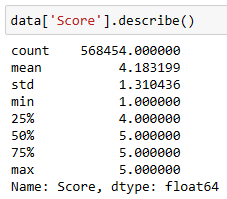
\includegraphics[scale=1]{assets/describe.PNG}
    \caption{Statistiques descriptives pour l'attribute Score}
    \label{fig:describe}
\end{figure}
\newpage
La sortie de la commande data['Score'].describe() pour la colonne 'Score' révèle que l'ensemble de données compte un total de 568,454 observations. La moyenne des scores est d'environ 4.18, avec un écart type de 1.31, indiquant une certaine variabilité dans les évaluations. Les scores varient de 1 à 5, avec 25\%, 50\%, et 75\% des scores situés à 4, 5, et 5 respectivement. Ces statistiques suggèrent une concentration des scores autour des valeurs élevées, avec une moyenne de 4.18 et une médiane de 5, suggérant une tendance positive dans les évaluations, probablement indicative d'une satisfaction générale des utilisateurs.

\subsubsection{Vérification des valeurs manquantes ou d'incohérences}
\begin{figure}[h]
    \centering
    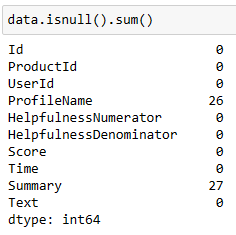
\includegraphics[scale=1]{assets/isnull.PNG}
    \caption{Détection d'Incohérences et de Manques de Données}
    \label{fig:isnull}
\end{figure}
La sortie obtenue à partir de la commande \texttt{data.isnull().sum()} présente le nombre de valeurs manquantes pour chaque colonne de l'ensemble de données. Un résumé de ces résultats est le suivant :

\begin{itemize}
    \item Pour les colonnes 'Id', 'ProductId', 'UserId', 'HelpfulnessNumerator', 'HelpfulnessDenominator', 'Score', et 'Time', aucune valeur manquante n'est à signaler.
    \item Cependant, la colonne 'ProfileName' présente 26 valeurs manquantes, tandis que la colonne 'Summary' en compte 27.
\end{itemize}

Cette information précise quelles colonnes spécifiques contiennent des valeurs manquantes et quantifie ces manques. Cette connaissance est cruciale pour déterminer la meilleure approche de gestion des données manquantes, que ce soit en les supprimant, en les remplaçant par des valeurs par défaut, ou en appliquant d'autres méthodes de gestion en fonction du contexte de l'analyse.

\newpage 
\subsubsection{Vérifier les valeurs uniques dans chaque colonne}
\begin{figure}[h]
    \centering
    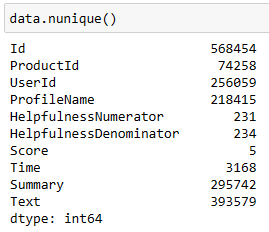
\includegraphics[scale=1]{assets/nunique.PNG}
    \caption{Verifier les valeurs uniques dans chaque colonne}
    \label{fig:isnull}
\end{figure}
La commande \texttt{data.nunique()} révèle la diversité des valeurs dans chaque colonne de l'ensemble de données. Les résultats montrent des variations significatives, allant de 5 valeurs uniques dans la colonne 'Score', indiquant une échelle de notation restreinte, à 393579 valeurs uniques dans la colonne 'Text', soulignant la grande variété de textes présents. Ces statistiques offrent un aperçu de la distribution des valeurs et de la portée de la diversité dans chaque attribut.

